\section{Evaluation}
\label{sec:evaluation}

Armed with the results of Sections~\ref{sec:algorithm}
and~\ref{sec:correctness}, we decided to benchmark the algorithm on a
test suite of carefully crafted pairs of types. This test suite was constructed by
gathering pairs of types that emerged from examples we have studied
and from programs we have written in FreeST, the programming language
for context-free session
types~\cite{almeida.etal_freest-functional-language}. 
During this process, we came across 
some types
%
%\begin{gather*}
%    \mu X . \&\{ \mathsf{Add}\colon X;X; !\intk,
%    \mathsf{Const}\colon ?\intk;!\intk,
%    \mathsf{Mult}\colon X;X;!\intk \}
%    \\
%    \mu Y . \&\{ \mathsf{Add}\colon Y;Y,
%    \mathsf{Const}\colon ?\intk,
%    \mathsf{Mult}\colon Y;Y \}; !\intk
%\end{gather*}
%
on which our algorithm took more than one hour
to terminate. This was not a reasonable running time for small 
types such as: 
$\mu X . \&\{ \mathsf{a}\colon X;X; !\intk,
    \mathsf{b}\colon ?\intk;!\intk,
    \mathsf{c}\colon X;X;!\intk \}$
and 
$\mu Y . \&\{ \mathsf{a}\colon Y;Y,
    \mathsf{b}\colon ?\intk,
    \mathsf{c}\colon Y;Y \};$ $ !\intk$.
%This is certainly not a reasonable
%running time for such small pair of types. 
Hence, we
looked into ways for improving the performance of the algorithm. 
We implemented the
following variants: 
\begin{enumerate}
	\item {\bf Eliminating redundant productions in the grammar} \\
	Realising that the size of 
	the expansion tree depends, among other
	things, on the number of productions in the grammar, we looked into
	ways of generating smaller grammars. Rather than blindly adding a new production
$Y \rightarrow \vec Z$, we look, in the set of productions, for a
production $W \rightarrow \vec X$ such that the language generated
from $\vec Z$ coincides with that from $\vec X$. In this
case, we add no new production and return the non-terminal~$W$ instead. To
find~$W$, we look for the least fixed-point of
sets of words in the
languages generated by $\vec Z$ and $\vec X$,
obtained with the same transition labels,
and compare them.
	\item {\bf Using a double-ended queue to prepend promising children} \\
A double-ended queue allows prioritizing nodes with potential to
reach an empty node faster.
The algorithm prepends (rather than
appends) nodes already empty or whose pairs $(\vec X, \vec Y)$
are such that $|\vec X|\leq 1$ and $|\vec Y| \leq 1$. 
	\item {\bf Using a filtering rule that removes nodes with hopeless pairs}\\
	A filtering rule
ensures that nodes composed by pairs of types with different norms (if normed)
are removed from the expansion tree, since these types are not equivalent. 
Notice that the filtering rule preserves the results of soundness and 
completeness.
	\item {\bf Iterating the simplification stage until a fixed point is reached}\\
	Iterating the simplification procedure on a given node $N$, the
algorithm computes the simplest possible children nodes derived from
$N$. Of course, we need to make sure that a fixed-point exists, which
we do with Theorem~\ref{thm:fixed_point}.
\end{enumerate}

\begin{theorem}
  \label{thm:fixed_point}
  The simplification function that results from applying the
  reflexive, congruence, \BPA, and filtering rules, has a fixed point
  in the complete partial ordered set of pairs node-ancestors, where
  the set of ancestors is 
  %supposed to be 
  fixed.
\end{theorem}
%
\begin{proof}
For the proof, consider the order $\leqSets$, defined on the
  $\text{\lstinline{Set (Node, Ancestors)}} \times
  \text{\lstinline{Set (Node, Ancestors)}}$, as $s_1 \leqSets s_2$ if
  there exists an injective map
  $\sigma : s_1 \rightarrow s_2$ s.t.\ $\sigma(n_1,a) = (n_2,a)$ with
  $n_2\subseteq n_1$. We prove that $\leqSets$ is a partial order and the 
  the simplification function is order-preserving. 
  We conclude that $(\text{\lstinline{Set (Node, Ancestors)}}, \leqSets)$ is
  a complete lattice and use Tarski's fixed point 
  theorem~\cite{tarski1955lattice}, to
  ensure that the simplification function has a fixed point in
  \lstinline{Set (Node, Ancestors)}.
  We omit the details due to space restrictions.
%  \vv{where do we place the proof? Also, added one more rule:
%    filtering. Do we still have a theorem?}
\end{proof}

The optimisations we propose aim at improving the performance of the
algorithm, however the branching nature of the expansion tree promotes
an exponential complexity: each simplification step (potentially)
generates a polynomial number of nodes, each of which with linear size
on the size of the input.  In turn, the same simplification phase may,
in the worst case, be iterated a linear number of times on the size of
the input.  For these reasons the complexity turns out to be (at least)
exponential.  
%Nevertheless, these heuristics seem to work quite well
%in practice, as we show in the next section.
%We tested these optimisations, to evaluate how would the algorithm
%perform in practice with the proposed heuristics.
To have a better understanding of how the algorithm would perform
in practice, we tested all the proposed optimisations. We evaluate 
each optimisation 1-4 individually (denoted by B1-B4, respectively)
and the gradual inclusion of optimisations, by the order in which they were
introduced above (cases B12, B123, B1234).
B0 stands for the base algorithm without any optimisation, $\BisimT$.

%Both for testing and for performance evaluation, we require a test
%suite. We started with a carefully crafted, manually produced, suite
%of valid and invalid tests. This test suite was constructed by
%gathering pairs of types that emerged from examples we have studied
%and from programs we have written in FreeST, the programming language
%for context-free session
%types~\cite{almeida.etal_freest-functional-language}.
% This suite comprised of a total os 169 valid and invalid tests.  The
% primary purpose of this preliminary evaluation step was to confirm
% the algorithm would be able to handle manual examples that we knew
% would emerge from real programs and examples. The algorithm
% succeeded in evaluating all the tests in due time.
%The tests produced by the method, although small and lacking diversity
%have revealed run times longer then we would expect for a compiler, as discussed
%in Section~\ref{sec:optimisations}. 
%The tests produced by this method are, on the one hand, small, and, on
%the other hand, lacking diversity.

The \emph{carefully crafted} test suite we have mentioned in the beginning
of this section is composed by small tests, lacking diversity.
So, we turned our attention to the automatic generation of test
cases. Generating pairs of arbitrary (well-formed) types that share no
variables is simple. The difficulty lies in deciding whether two such
types, independently generated, are bisimilar. Even if an oracle could
be identified, the probability that a randomly generated pair of types
turns out to be equivalent would be extremely low. Instead, we proceed
by generating arbitrary pairs of types that are bisimilar by
construction. Theorem~\ref{thm:axioms} naturally induces an algorithm:
given a natural number $n$ (the size of the pair), arbitrarily select
for the base case ($n=0$) one of the pairs in item 1 of the theorem
and for the recursive case ($n\ge1$) one of the pairs in 2--12 items.

\begin{theorem}[Properties of type equivalence]
\label{thm:axioms}
%\begin{multicols}{1}
{\small  \begin{enumerate}[leftmargin=*]
    % Congruence
  \item $\skipk \TypeEquiv \skipk$ and $\sharp B \TypeEquiv \sharp B$;
  \item $S;T \TypeEquiv U;V$ if $S \TypeEquiv U$ and $T \TypeEquiv V$;
  \item $\mu X.S \TypeEquiv \mu X.T$ if $S \TypeEquiv T$;
  \item $\star\{\ell_i\colon S_i\}_{i\in I}\TypeEquiv
    \star\{\ell_i\colon T_i\}_{i\in I}$ if $S_i \TypeEquiv T_i$ for each $i$;
    % Laws for sequential composition
  \item $S\TypeEquiv T;\skipk$ and $S\TypeEquiv \skipk;T$ if $S \TypeEquiv T$;
  \item $\star\{\ell_i\colon S_i\}_{i\in I};U\TypeEquiv
    \star\{\ell_i\colon T_i;V\}_{i\in I}$ if $(S_i \TypeEquiv T_i)_{i\in
      I}$ and $U \TypeEquiv V$;
  \item $T \TypeEquiv S$ if $S \TypeEquiv T$;
  \item $R;(S;T) \TypeEquiv (U;V);W$ if $R \TypeEquiv U$, $S \TypeEquiv V$, and $T\TypeEquiv W$;
    % Laws for mu-types
  \item
    $\mu X.\mu Y.S \TypeEquiv \mu X.\subs XYT \TypeEquiv \mu Y.\subs
    YXT$ if $S \TypeEquiv T$;
  \item $\mu X.S \TypeEquiv T$ if $S \TypeEquiv T$ and $x\notin\free(S)$;
  \item $\subs UXS\TypeEquiv \subs VXT$  if $S \TypeEquiv T$ and $U \TypeEquiv V$;
  \item $\mu X.S \TypeEquiv \subs{\mu X.T}{X}T$ if $S \TypeEquiv T$.
  \end{enumerate}}
 % \end{multicols}
\end{theorem}
%
\begin{proof}
  1--3: Bisimulation is a congruence. 4--12: Thiemann and
  Vasconcelos~\cite{thiemann2016context} exhibit the appropriate
  bisimulations.
\end{proof}

For evaluating the performance of the algorithm on non-bisimilar 
pairs we independently
generate two types, run function $\BisimT$ on them, and discard the
data collected in the rare event that the pair turns out to be
bisimilar.
%
For testing, however, we rely on manually crafted tests, given that a
solution based on anti-axioms does not work: bisimulation for
context-free session types is such that there are types
$S \not\bisim T$ such that $\mu X.S \bisim \mu X.T$ (just think of
$!\intk;X;X$ and $!\intk;X$).

We used QuickCheck~\cite{DBLP:conf/icfp/ClaessenH00} to generate two test
suites. That for bisimilar pairs (constructed based on
Theorem~\ref{thm:axioms}) comprises 1000 entries, featuring types with
a number of nodes (in the syntax tree) ranging from 1 to 35751. The
test suite for non-bisimilar pairs (constructed by independently
generating two types and verifying they were not equivalent) includes
1000 pairs with a number of nodes ranging from 1 to 387.\\
%
%The slowest negative test takes under 775Mb of RAM to execute.
%
  \begin{minipage}[b]{0.49\textwidth}
   {\small 
  \centering
 
	\begin{tabular}{ |c|c|c| }
	 \hline
 		Version &  {\color{MidnightBlue}Bisimilar} & {\color{orange}Not bisimilar}  \\ 
 		 \hline
	 	B0 & 5 & 0 \\  
	 	B1 &  1 & 0 \\ 
	 	B2 & 6 & 0 \\ 
	 	B3 &  12 & 0 \\
	 	B4 &  4 & 0 \\
	 	B12 &  2 & 0 \\   
	 	B123 &  6 & 0 \\
	 	B1234 &  \bf{0} & \bf{0} \\ 
	 	 \hline  
	\end{tabular}\vspace*{6mm}
	\captionof{table}{Number of timeouts for each optimisation and for both test 
	suites.\label{table:timeouts}\vspace*{4mm}}
	}
	\end{minipage}
	\hfill
\begin{minipage}[b]{0.49\textwidth}
 {\small 
\centering
    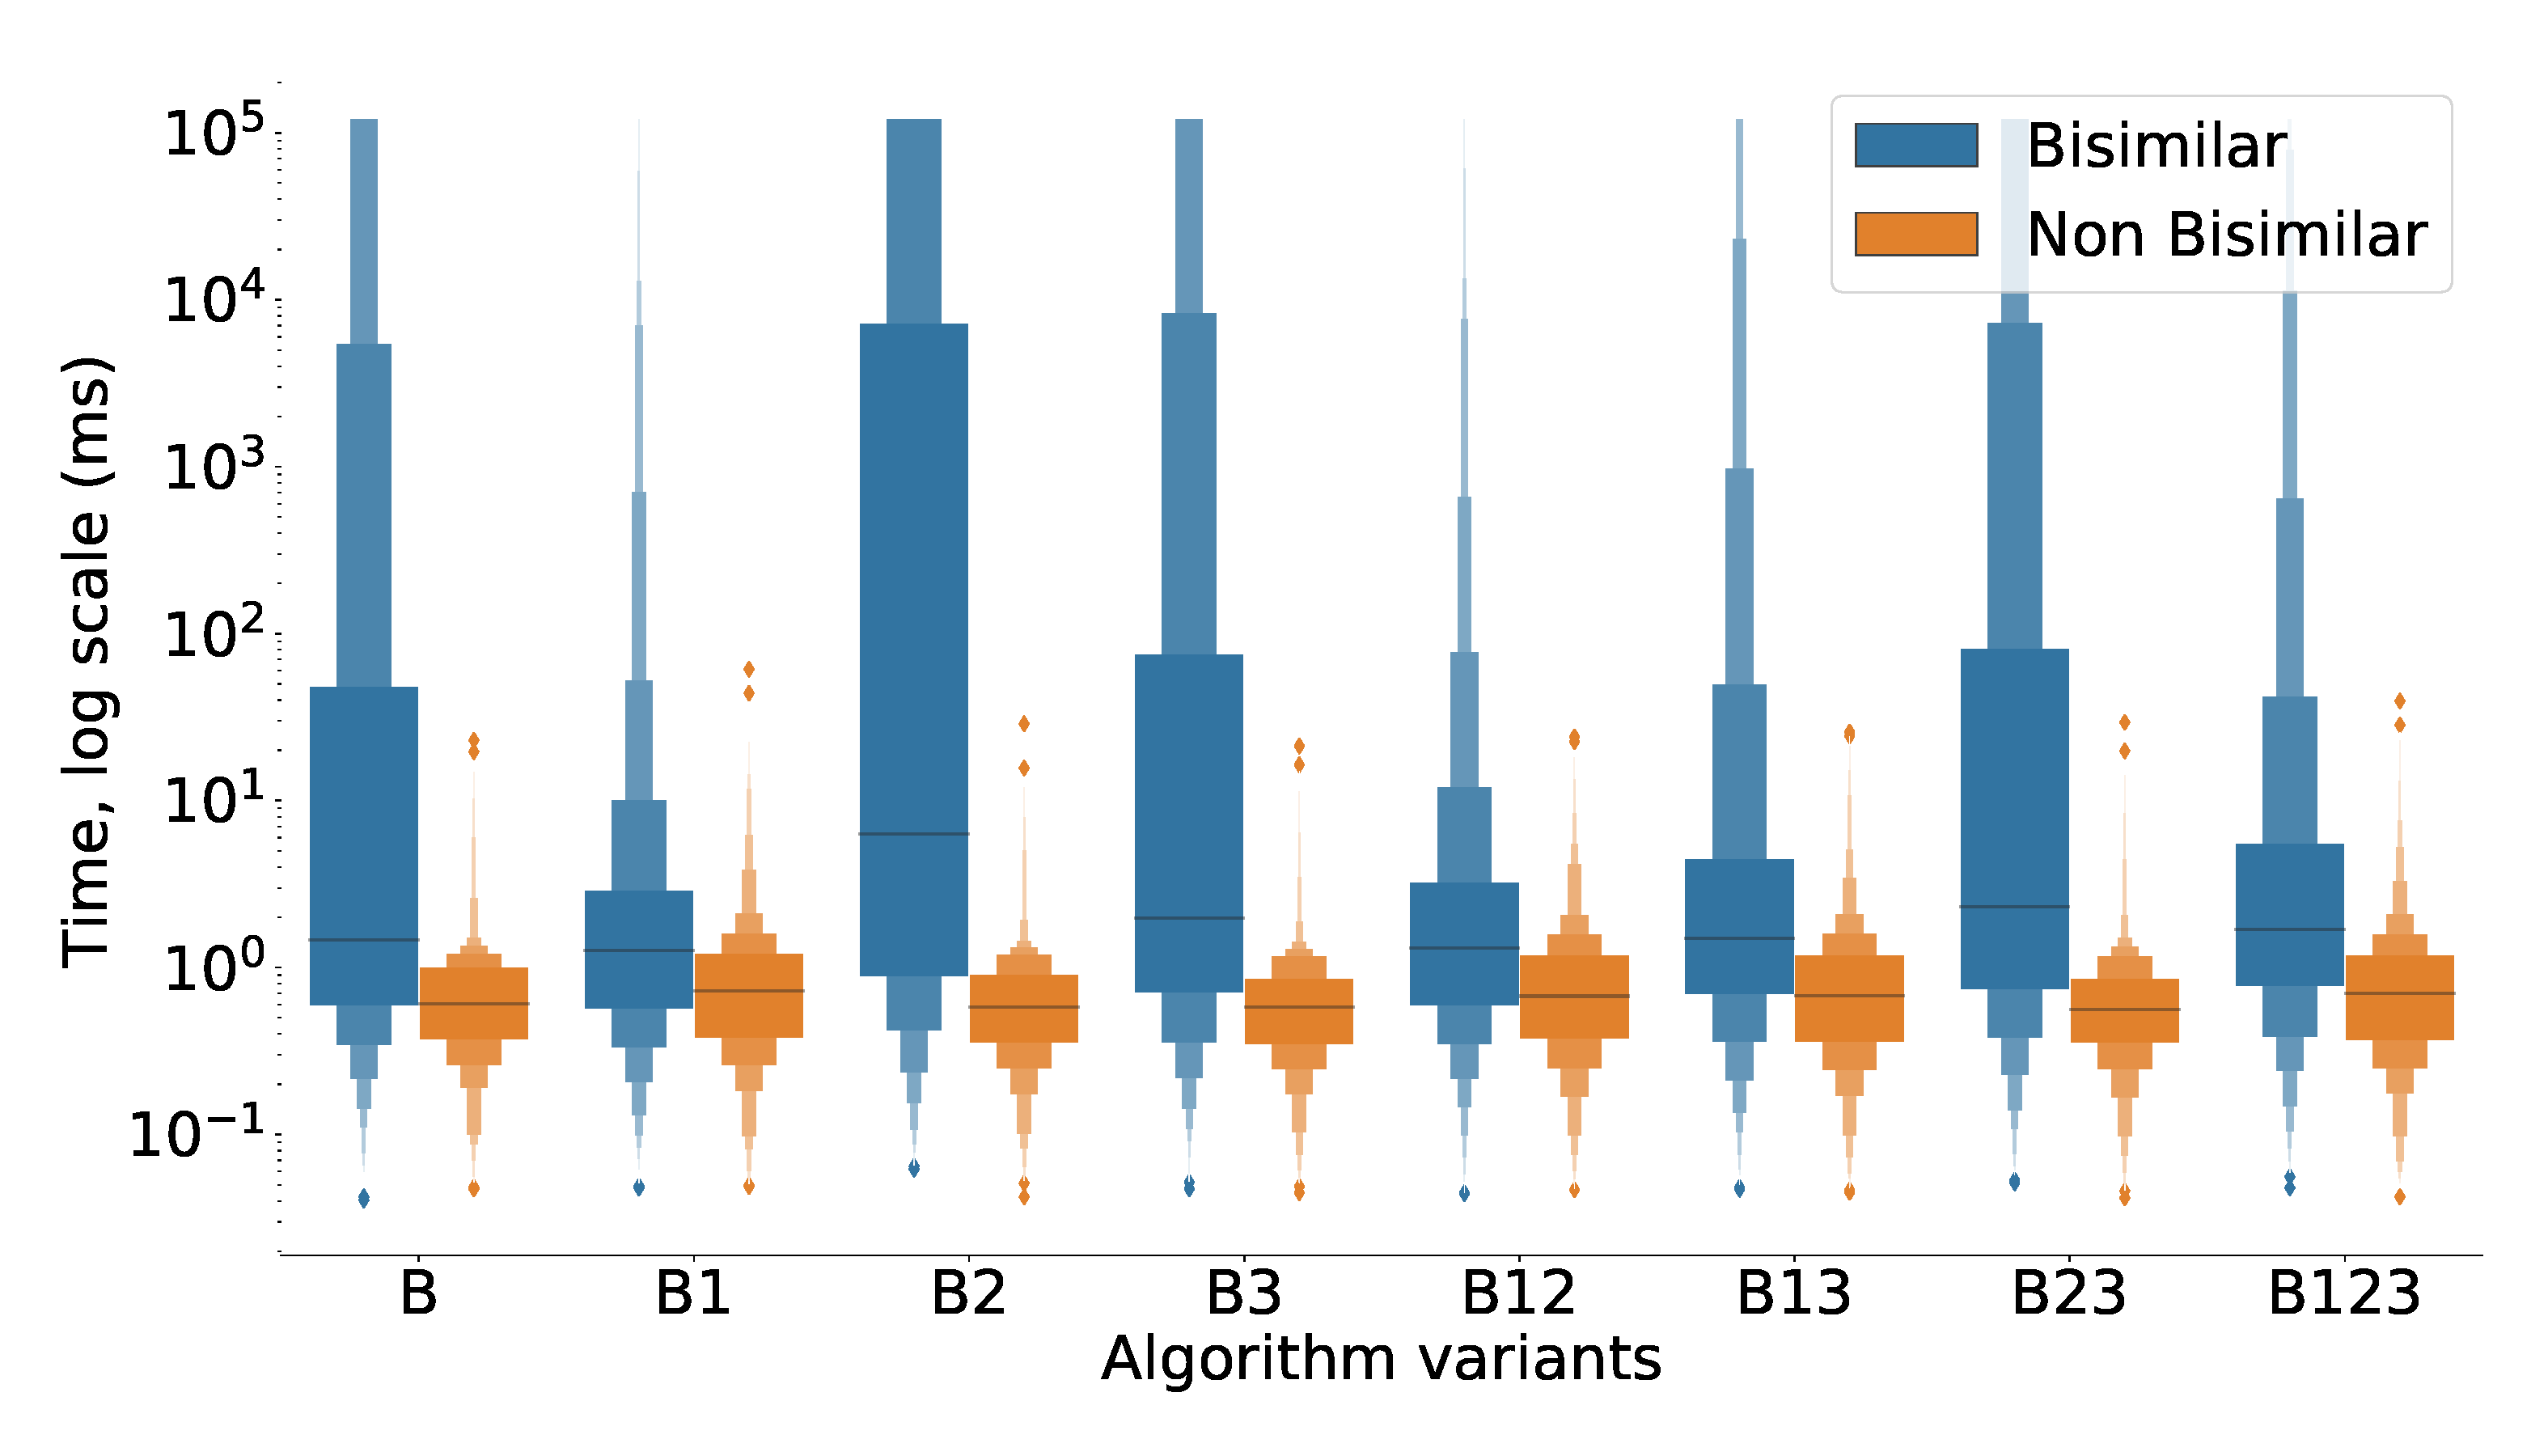
\includegraphics[height=.85\textwidth]{img/distribution_boxplot}%
    \captionof{figure}{Distribution of execution time of function $\BisimT$ for both test suites. 
    Both scales are logarithmic.\label{fig:results}}}
    %\caption{Distribution of the execution time. \label{fig:results}}
\end{minipage}
	%\caption{Number of timeouts for each optimisation.\label{table:timeouts}}
    %
%    \caption{The test suite composed by equivalent pairs of types is represented in blue and the
%    test suite with non-equivalent pairs of types is represented in orange. Time 
%    in microseconds, $\mu s$. Both scales are logarithmic.\\
%    (a) Distribution of execution time of function $\BisimT$ for both test suites.\\
%    (b) Number of timeouts for each optimisation.\label{table:timeouts}
%    Distribution of execution time of function $\BisimT$ with all 
%    optimisations
%    per total number of nodes 
%    in the abstract syntax trees of the types.
%    }%
%    \label{fig:results}%
%\end{figure}


%\begin{figure}[t]
%    \centering
%    \subfloat[Distribution of the execution time]{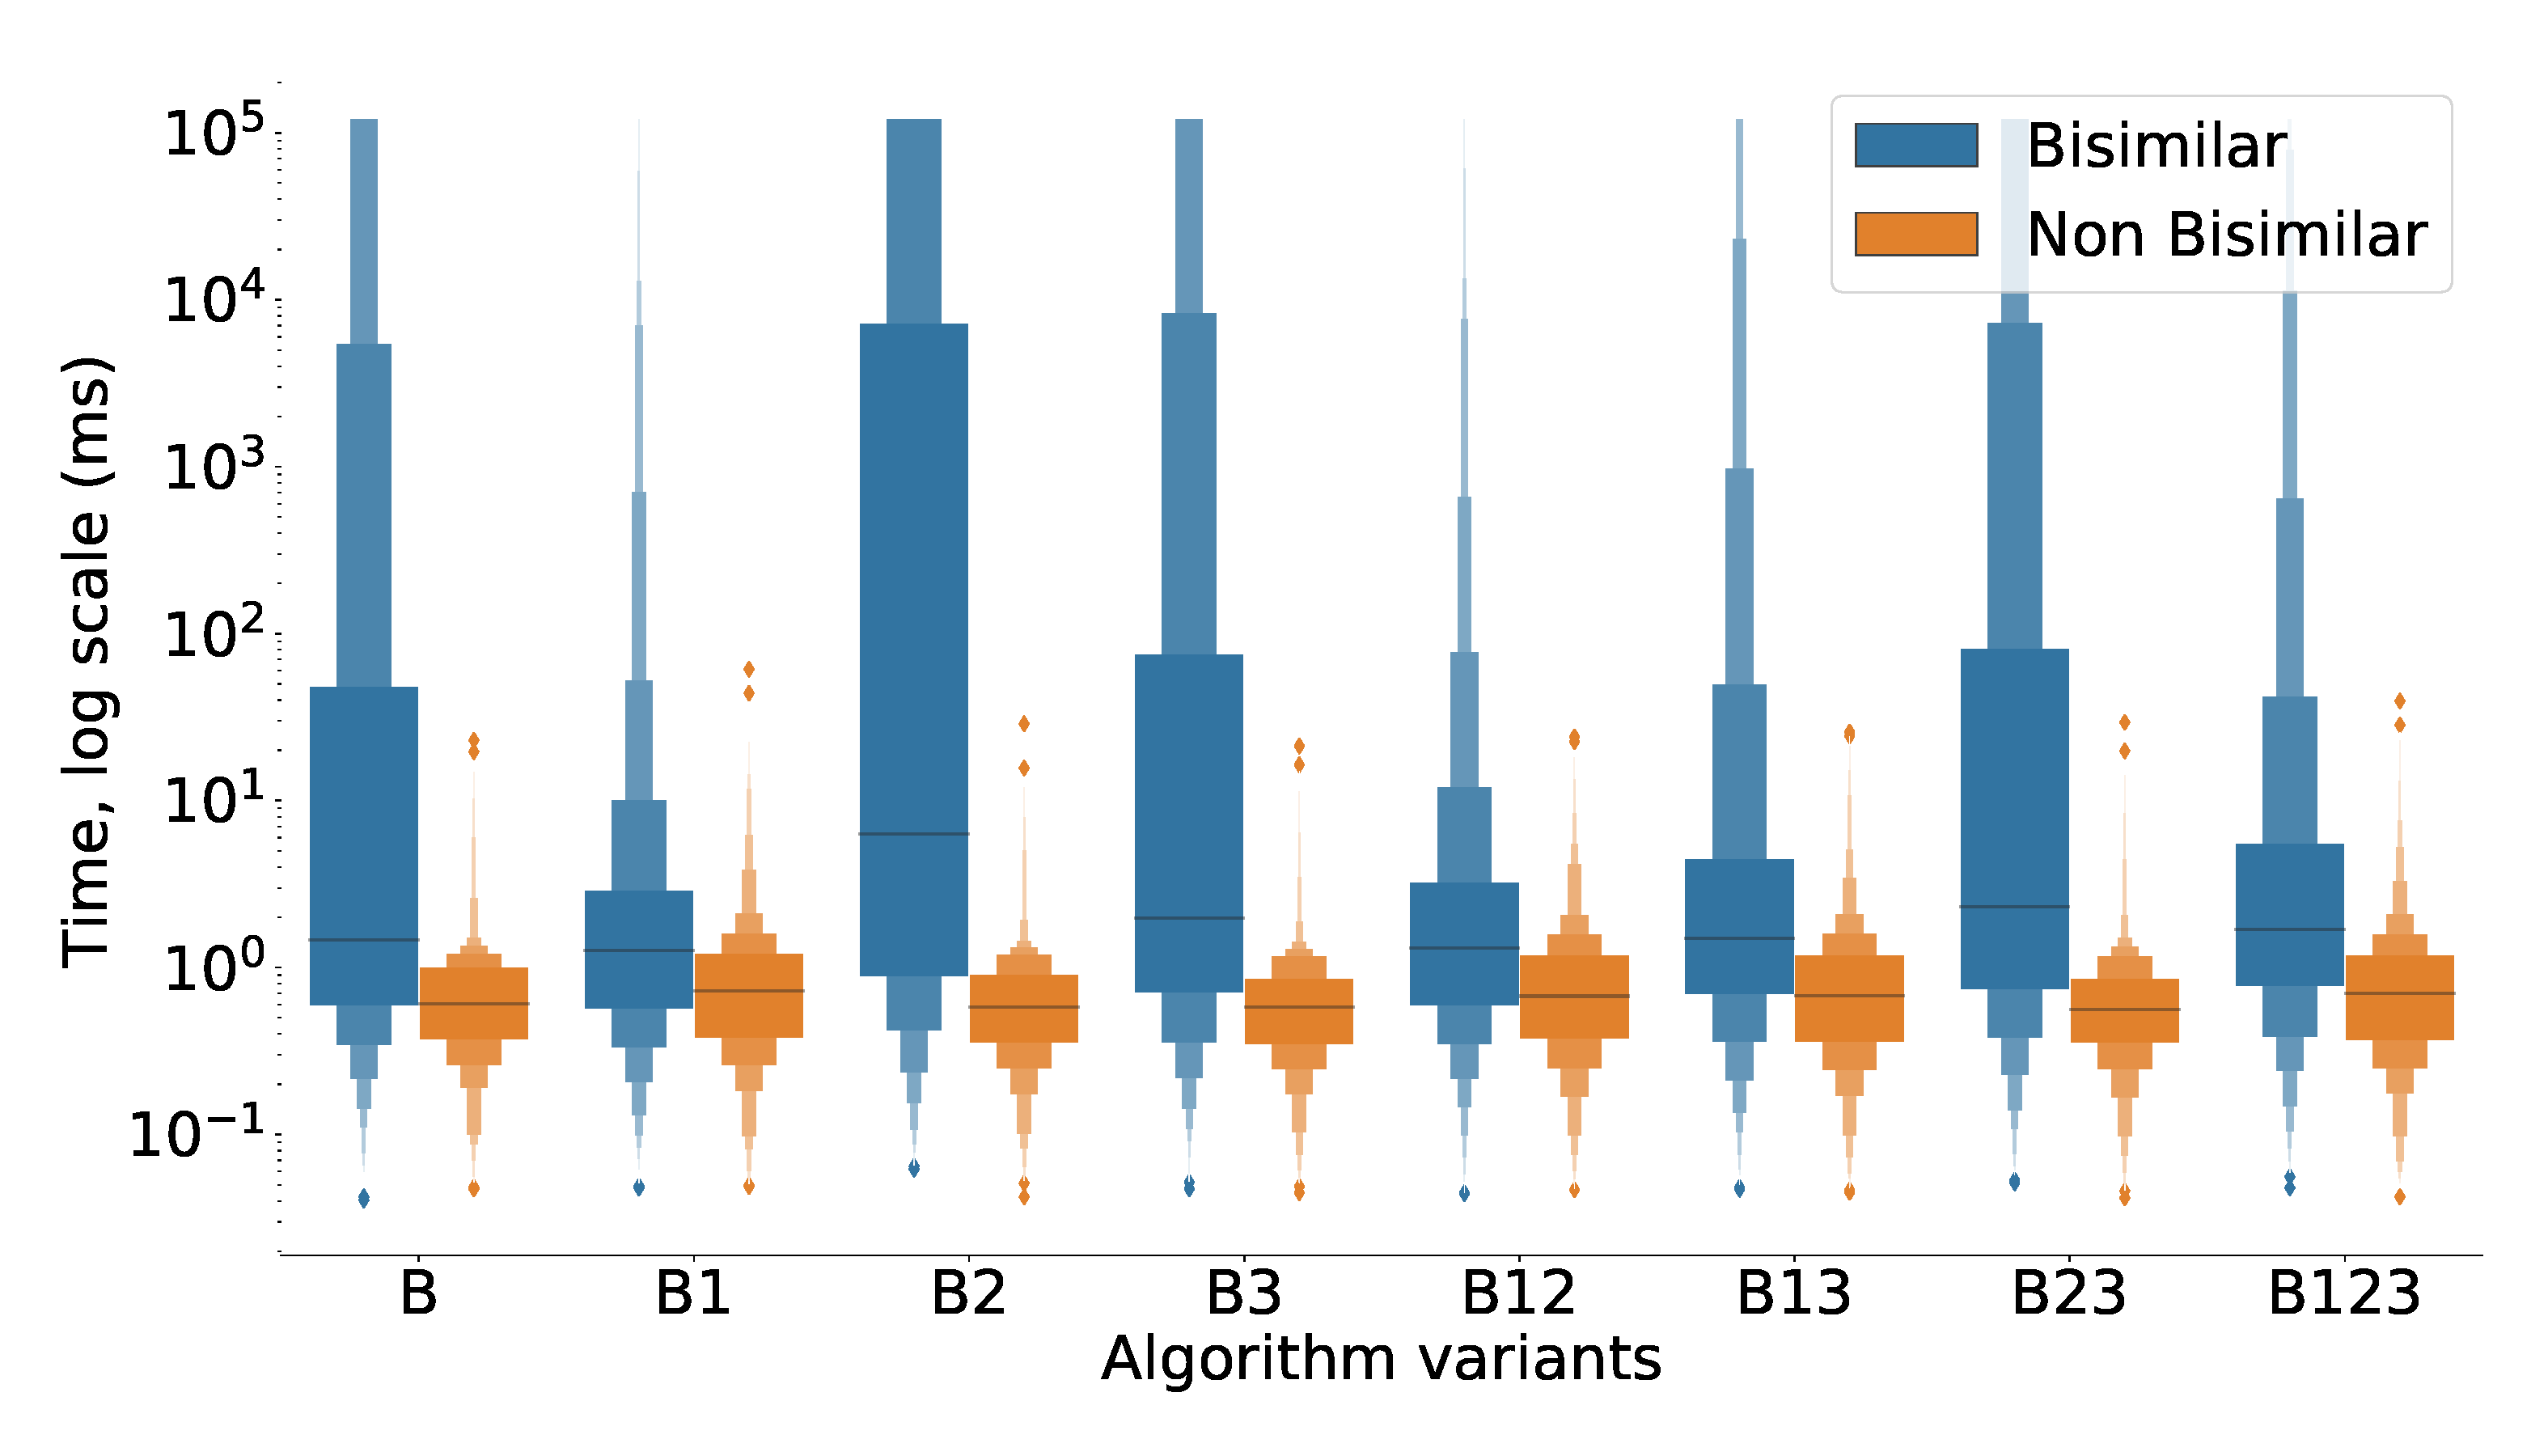
\includegraphics[height=.5\textwidth]{img/distribution_boxplot}}%
%    \subfloat[Execution time per number of nodes]{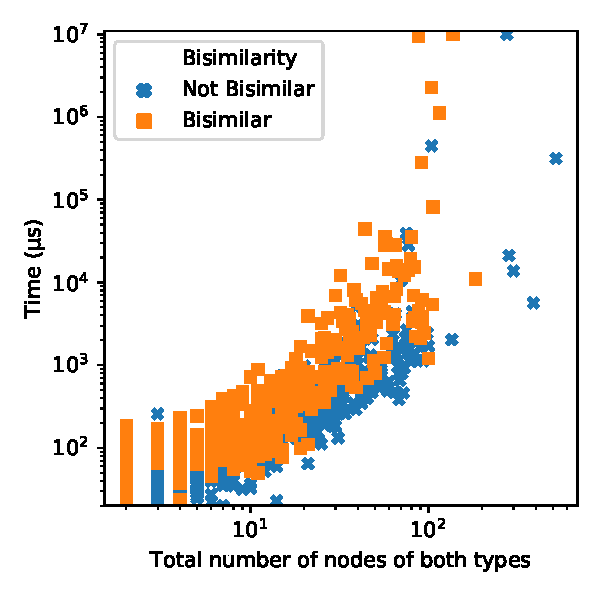
\includegraphics[height=.5\textwidth]{img/nodes_time_B1234}}%
%    \caption{The test suite composed by equivalent pairs of types is represented in blue and the
%    test suite with non-equivalent pairs of types is represented in orange. Time 
%    in microseconds, $\mu s$. Both scales are logarithmic.\\
%    (a) Distribution of execution time of function $\BisimT$ for both test suites.\\
%    (b) Distribution of execution time of function $\BisimT$ with all 
%    optimisations
%    per total number of nodes 
%    in the abstract syntax trees of the types.}%
%    \label{fig:results}%
%\end{figure}

%\begin{figure}[h]
%\centering
%	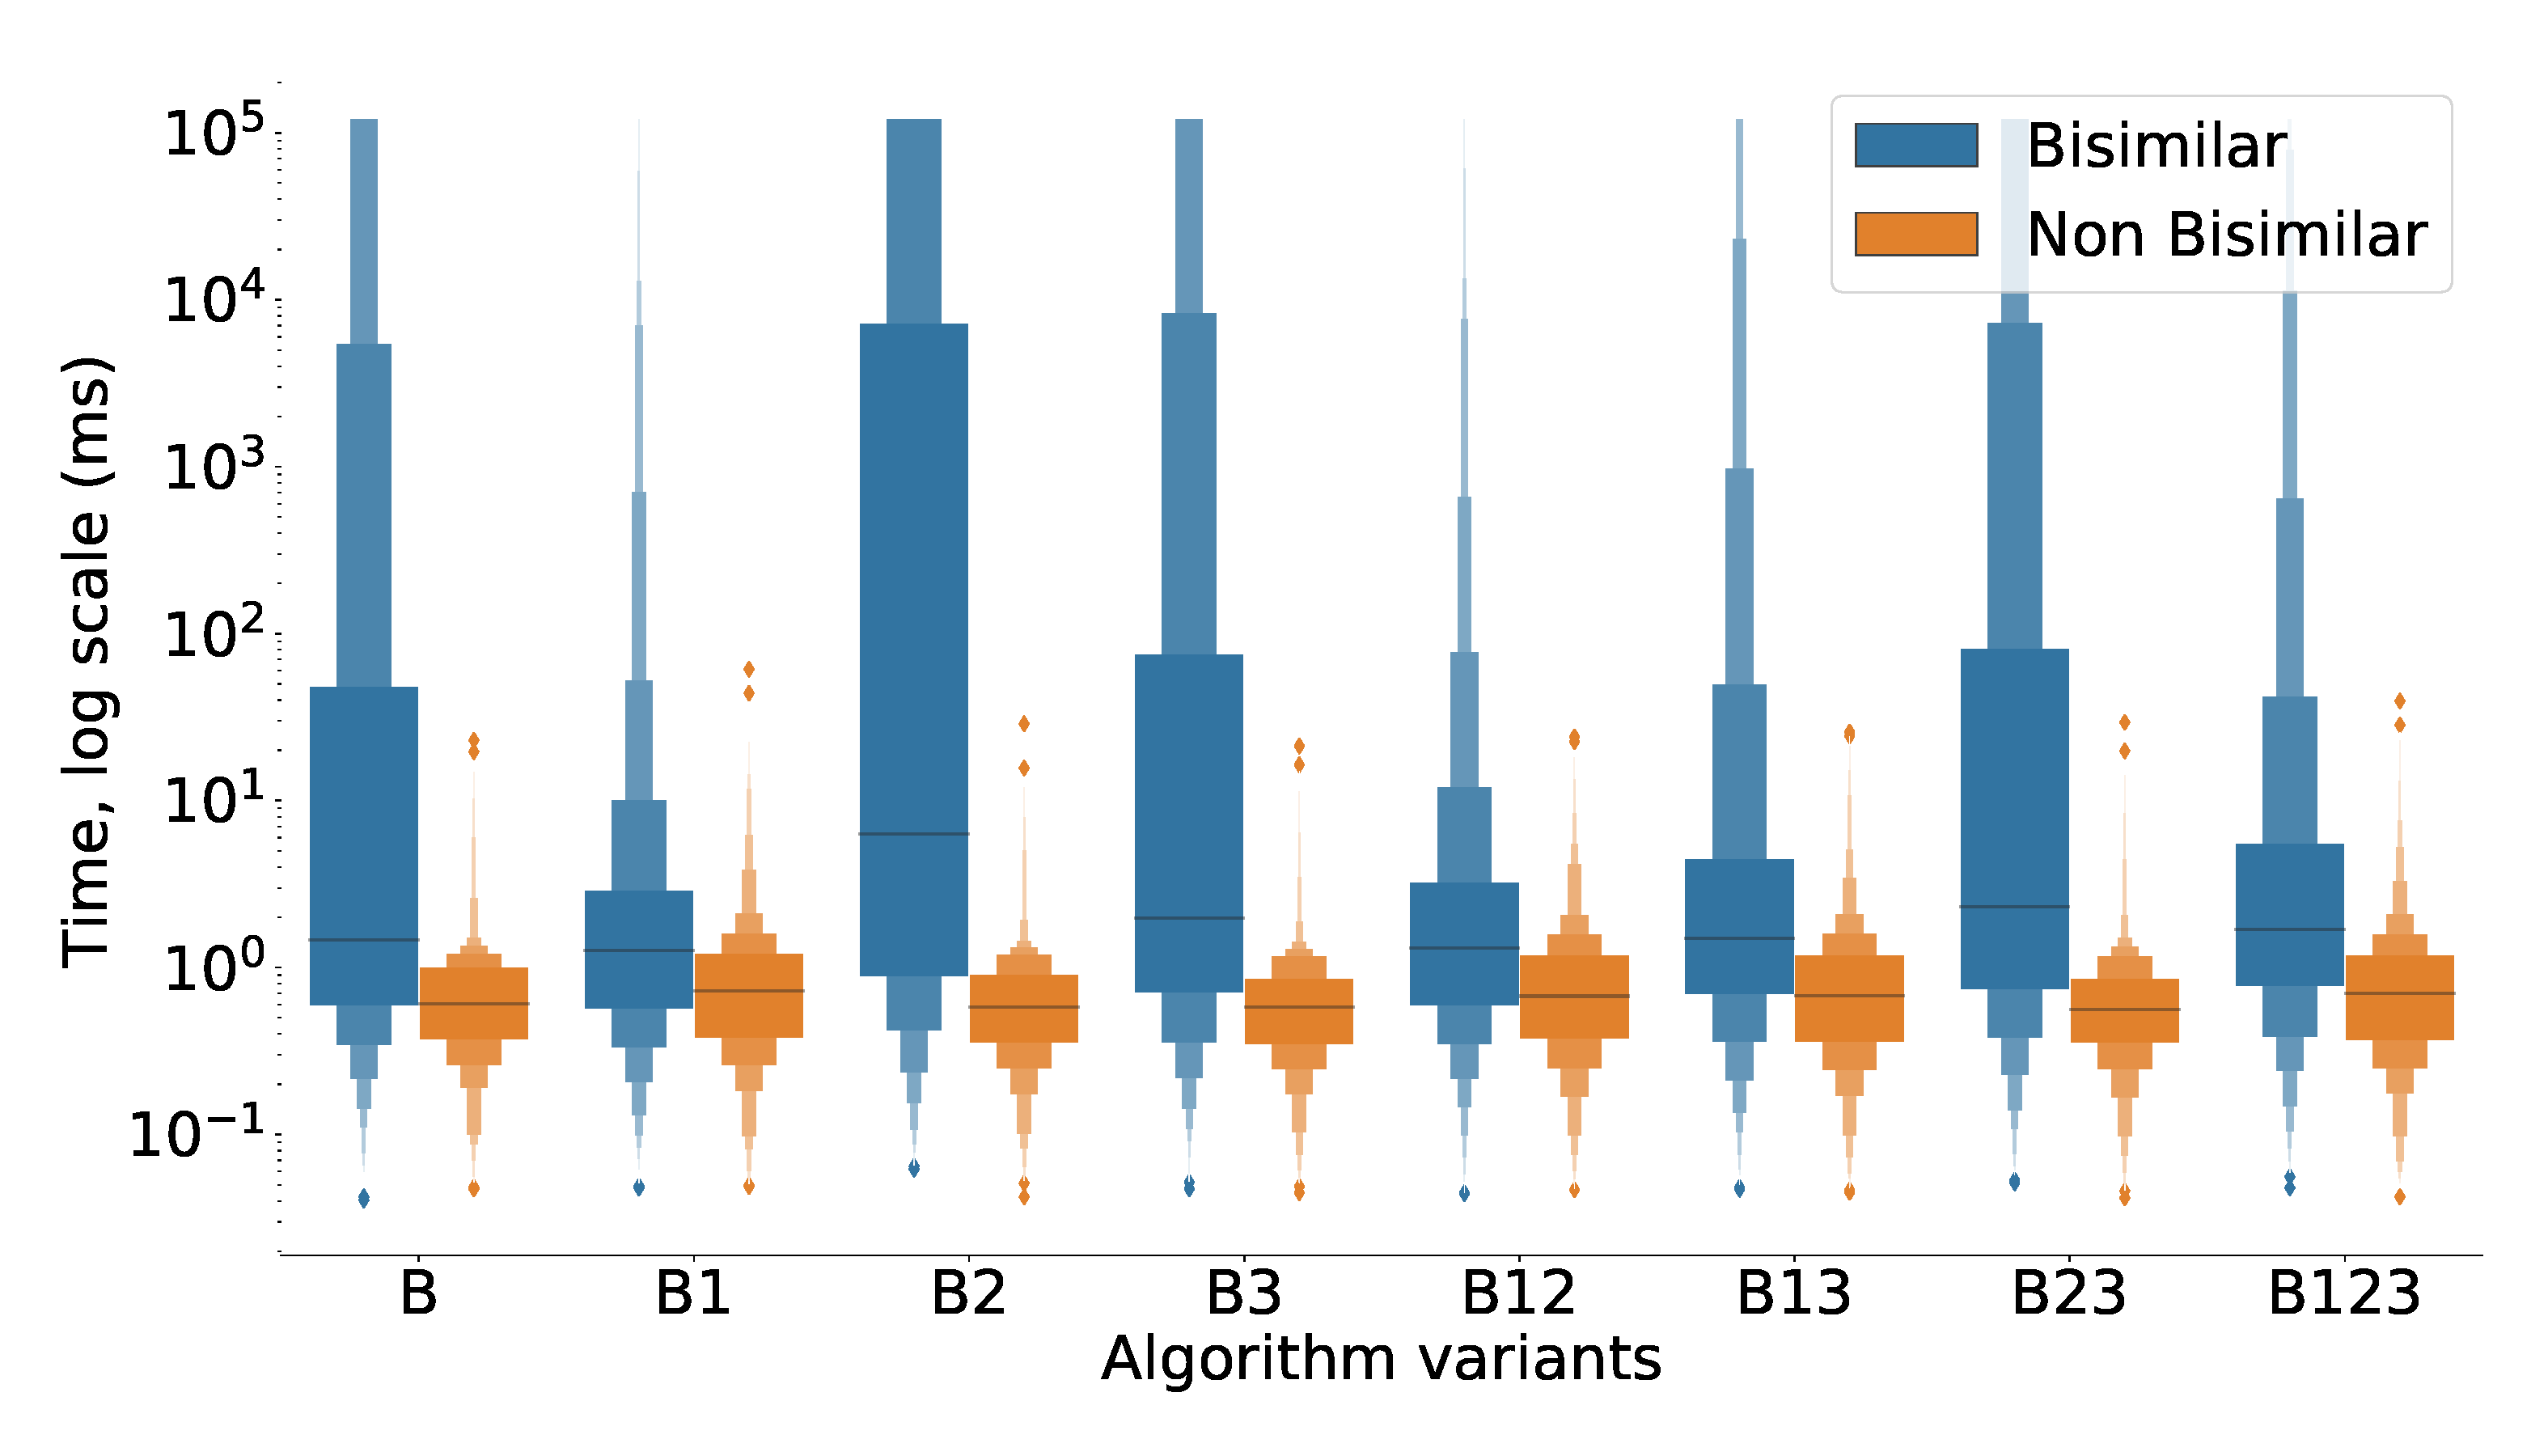
\includegraphics[height=6cm]{img/distribution_boxplot}	\hspace*{2mm}
%	\caption{Distribution of execution time of function $\BisimT$ for the 
%	test suite with equivalent pairs of types (blue, at the top) and for the 
%	test suite with non-equivalent pairs of types (orange, at the bottom).
%	Time is represented in microseconds, $\mu s$.}
%	\label{fig:run_times}
%\end{figure}
%\begin{figure}[h]
%\centering
%	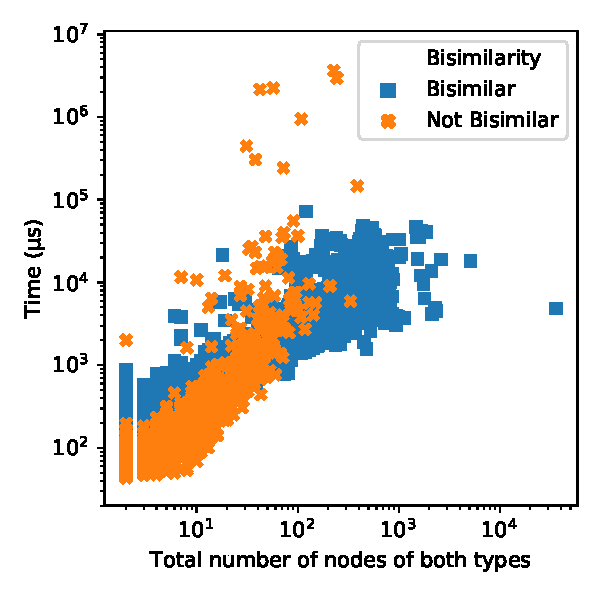
\includegraphics[height=6cm]{img/nodes_time_B0}
%	\caption{Distribution of execution time per total number of nodes for
%	equivalent and non-equivalent pairs of types (represented by blue and
%	orange, respectively). Time is represented in microseconds, $\mu s$.}
%	\label{fig:nodes_vs_time}
%\end{figure}

We implemented the algorithm described by the function $\BisimT$ 
and the proposed optimisations
in
%300 lines of 
Haskell and used the Glasgow Haskell Compiler (version
8.6.5), provided by the docker image
\texttt{fpco/stack-build}. 
Evaluation was conducted on a machine with
an Intel Xeon X5670 at 2.93GHz and 24 GB of RAM.
%We evaluated the algorithm for each optimisation individually, and for the 
%gradual inclusion of optimizations, by the order in which
%they were introduced above.
We ran the tests with a timeout of 30 minutes. 

Table~\ref{table:timeouts} 
exhibits the number of timeouts for each version of the algorithm for both
test suites. 
Although we do not observe an improvement with the gradual
inclusion of optimisations in the order we have chosen,
we achieve 0 timeouts when all the optimisations are included.
%
%\begin{table}
%\centering
%	\begin{tabular}{ |c|c|c|c| }
%	 \hline
% 		Version ID & Version description & Bisimilar test suite & Not bisimilar 
% 		test suite \\ 
% 		 \hline
%	 	B0 & \text { base case}& 5 & 0 \\  
%	 	B1 & \text { reuse productions}& 2 & 1 \\ 
%	 	B2 & \text { use double-ended queue}& 6 & 0 \\ 
%	 	B3 & \text { use filtering}& 12 & 0 \\
%	 	B4 & \text { iterate simplification}& 4 & 0 \\
%	 	B12 & \text {case B1 + case B2}& 3 & 1 \\   
%	 	B123 & \text {case B12 + case B3}& 7 & 1 \\
%	 	B1234 & \text {case B123 + case B4}& \bf{1} & \bf{1} \\ 
%	 	 \hline  
%	\end{tabular}
%	\caption{Number of timeouts for each optimisation.\label{table:timeouts}}
%\end{table}
%
%
Figure~\ref{fig:results} depicts the distribution of the execution
times (in $\mu s$) for both test suites and for all optimisations. 
In this plot, we observe the distribution of tests for each execution time.
All the versions exhibit similar execution times for the majority 
of the tests.
Although we have carried out extensive tests, we remark that, when used 
in a compiler, the algorithm will mostly come across types with a reduced 
number of nodes in the abstract syntax tree.

%\begin{figure}[h]
%	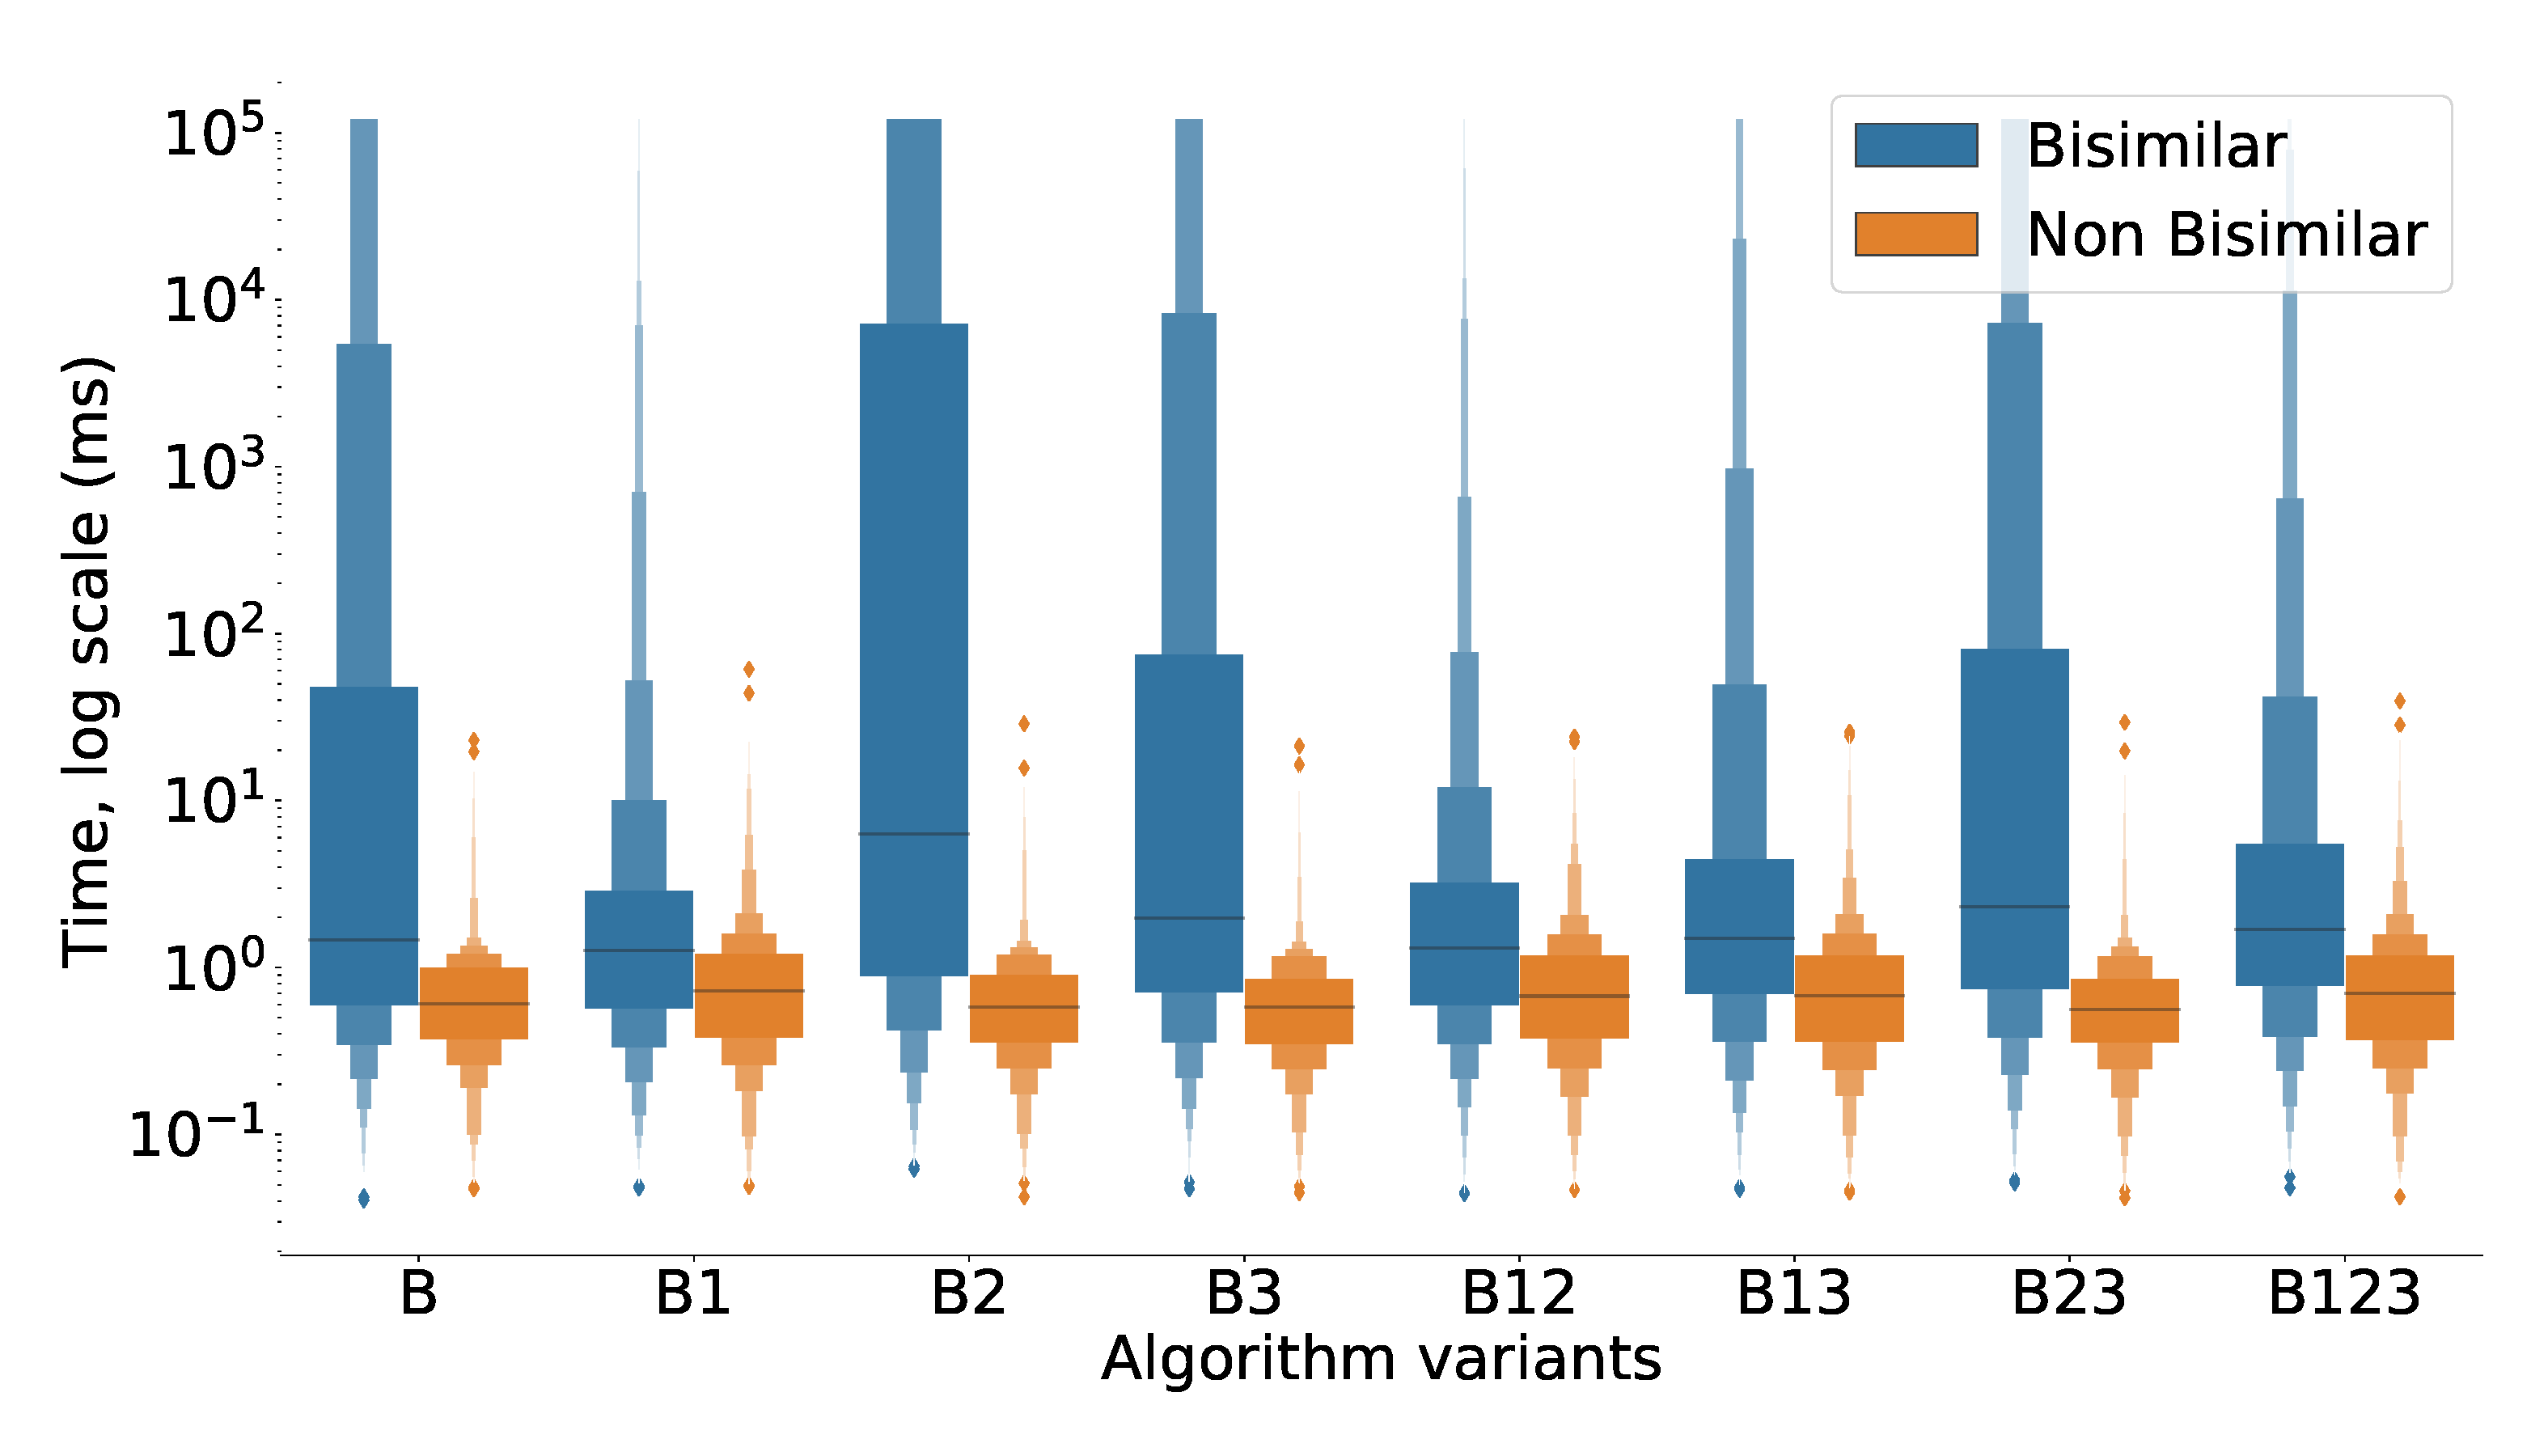
\includegraphics[height=6cm]{img/distribution_boxplot}	\hspace*{2mm}
%	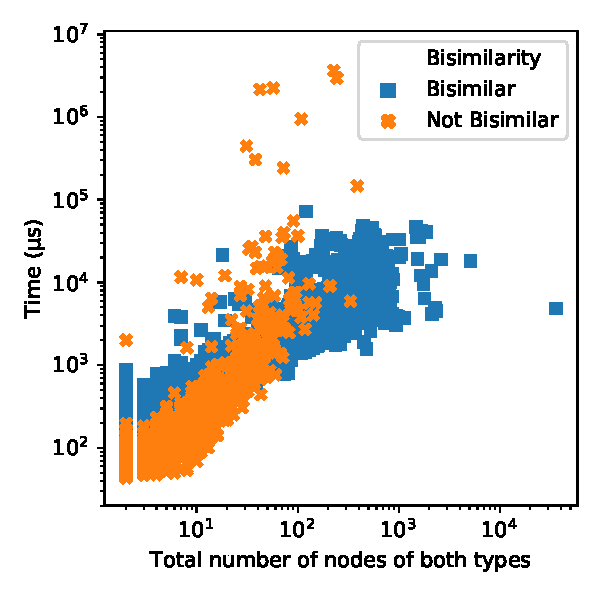
\includegraphics[height=6cm]{img/nodes_time_B0}
%	\caption{Distribution of execution time of function $\BisimT$ (on the left) and distribution of execution time per total number of nodes of both types (on the right).}
%	\label{fig:results}
%\end{figure}


%Figure~\ref{fig:results} (b) represents the distribution of execution
%time per total number of nodes in the abstract syntax trees of the
%types. We observe an exponential increase in the
%runtime with the number of nodes, as expected due to the nature of the
%expansion tree.
% We suspect that if we had carried out tests with a larger number of
% nodes, we would also have had observed an exponential growth in the
% execution time.

%Although the runtime of $\BisimT$ is good enough for justifying its
%inclusion in a compiler, we identified a few potential optimisations
%and analysed their impact on the execution time. We implemented the
%following variants: i) eliminating redundant productions in the
%grammar, ii) using a double-ended queue where promising children are
%prepended rather than appended, iii) adding a filter rule to
%simplification stage that removes hopeless pairs from nodes, and iv)
%iterating the simplification stage until a fixed point is reached.
%%
%Running the test suite discussed above on these variants, alone and
%in different combinations, we found no decrease in the runtime.

% Once the improvement proposals were established, we benchmarked the
% algorithm on a test suite of carefully crafted pairs of types
% based on cases observed when using the compiler where the algorithm is
% used~\cite{almeida.etal_freest-functional-language}. These
% tests comprise valid and invalid equivalences, for a total of 154
% tests. We have profiled our program for the time and memory allocated
% during the tests. For this purpose, we have used GHC's profiling
% feature, that maintains a cost-centre stack to keep track of the
% incurred costs. The results are depicted in
% Figure~\ref{fig:results}.

% \begin{figure}[h]
% 	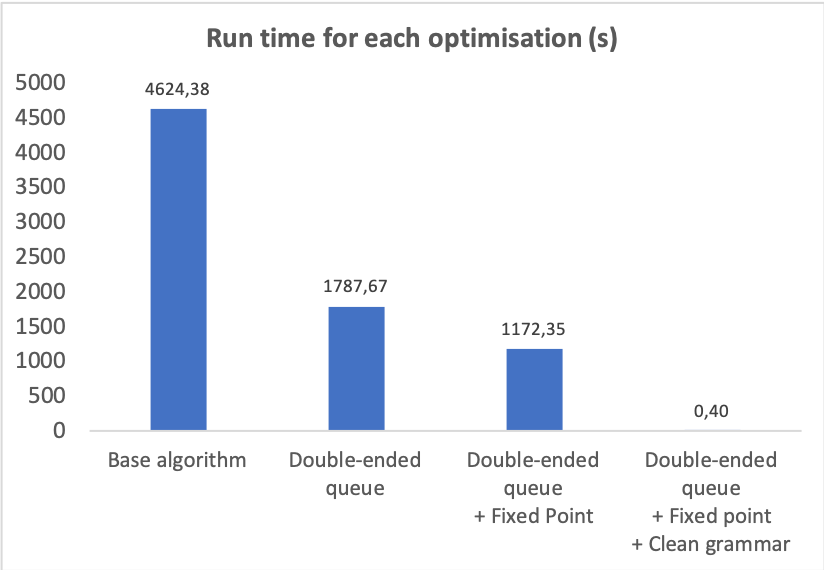
\includegraphics[height=4cm]{img/run_time}	\hspace*{2mm}
% 	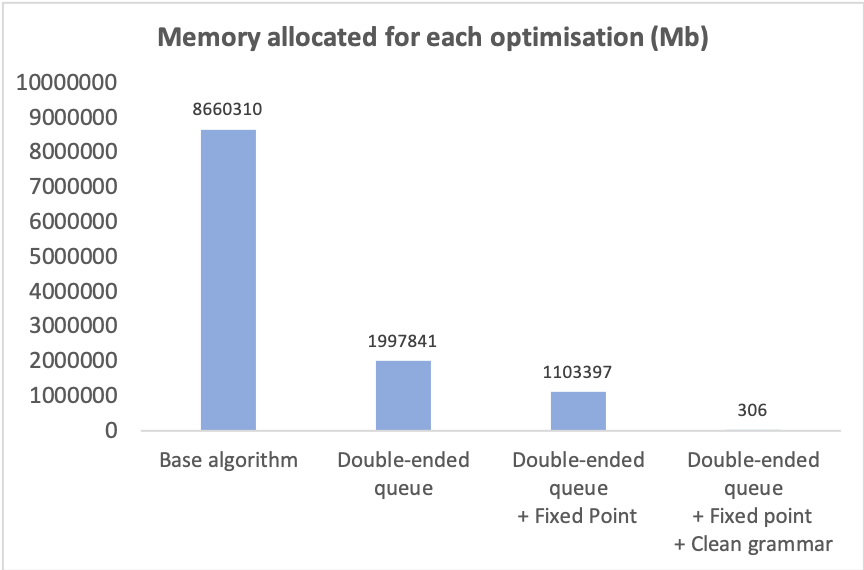
\includegraphics[height=4cm]{img/memory_alloc}
% 	\caption{Test results: running times (on the left) and
% 	memory allocated (on the right) checking the equivalence
% 	of context-free session types in 154 tests.}
% 	\label{fig:results}
% \end{figure}

% For the base algorithm, proposed in Listing~\ref{lst:algorithm}, we
% obtained a running time of about 4624 seconds and
% 8,660,309 Mb memory allocated. From the moment we introduced the
% optimizations the results improved remarkably:
% implementing a double-ended queue we reduced the running time to 1788
% seconds and the allocated memory to 1,997,841 Mb, by also
% iterating the
% simplification phase in the search for a fixed point we decreased these values
% to a running time of 1172 seconds and
% allocated memory of 1,103,397 Mb. The
% combination of these enhancements with the clean grammar generation
% exhibit an improvement in more than 1,000,000\% from the base case,
% achieving a running time of 0.4 seconds and 306 Mb
% of memory allocated.

% %iterating the
% %simplification phase in the search for a fixed point allowed to reduce
% %the running time to 110.35 seconds and the memory allocated to 164,745
% %Mb, whereas the implementation of the double-ended queue allowed to
% %reduce the running time to 18.45 seconds and the allocated memory to
% %29,298. The combination of both exhibit an improvement on more than
% %1,000,000\% from the base case, achieving an average of 0.04
% %seconds for the running time and 62 Mb of allocated memory.

% We should also highlight that, we run example~\eqref{ex:chaotic}
% with the improved algorithm, in a battery of 100 runs, and obtained an
% average running time of 0.008 seconds.

% The heuristic we proposed actually circumvents the exponential complexity
% inherent to the expansion tree, thus allowing to obtain running times that
% are manifestly small and to use this algorithm as an integral
% part of a compiler, as we had intended from the beginning.

%%% Local Variables:
%%% mode: latex
%%% TeX-master: "main"
%%% End:
